%
\documentclass[referee]{aa} % for a referee version
%\documentclass[onecolumn]{aa} % for a paper on 1 column  
%\documentclass[longauth]{aa} % for the long lists of affiliations 
%\documentclass[letter]{aa} % for the letters 
%\documentclass[bibyear]{aa} % if the references are not structured 
%                              according to the author-year natbib style


%\documentclass{aa}  
\usepackage{hyperref}
\usepackage{graphicx}
%%%%%%%%%%%%%%%%%%%%%%%%%%%%%%%%%%%%%%%%
\usepackage{txfonts}
%\usepackage{multirow}
%%%%%%%%%%%%%%%%%%%%%%%%%%%%%%%%%%%%%%%%
\usepackage{subcaption}
\usepackage{flushend}
  % results heading (mandatory)
\begin{document} 


   \title{Data processing pipelines and the data platform for the X-ray spectrometer/imager STIX onboard Solar Orbiter}

   \subtitle{}

   \author{Hualin Xiao
          \inst{1}
          \and 
          Shane Maloney 
          \inst{2}
          \and S\"am Krucker\inst{1}
          \and Paolo Massa \inst{6}
          \and Ewan Dickson \inst{4}
          \and Lastufka Erica \inst{1}
          \and László Etesi \inst{1}
          \and Andrea Francesco Battaglia\inst{3}
          \and Nicky Hochmuth \inst{1}
          \and Frederic Schuller \inst{7}
          \and Ryan Daniel \inst{1}
          \and Collier Hannah \inst{1}
          \and Olivier Limousin \inst{5}
          \and Alexander Warmuth \inst{7}
          \and other contributors
         }

   \institute{University of Applied Sciences and Arts Northwestern Switzerland (FHNW), 5200 Windisch, Switzerland \\
              \email{hualin.xiao@fhnw.ch}
         \and
          Astrophysics Research Group, School of Physics, Trinity College Dublin, Dublin 2, Ireland
          \and
             ETH Z\"urich, R\"amistrasse 101, 8092 Z\"urich, Switzerland
         \and University of Graz, Universitätspl. 3, 8010 Graz, Austria
         \and IRFU, CEA, Université Paris-Saclay, and Université Paris Diderot, AIM, Sorbonne Paris Cité, CEA, CNRS, 91191 Gif-sur-Yvette,
         France
         \and Dipartimento di Matematica, Università degli Studi di Genova, Via Dodecaneso 35, 16146 Genova, Italy
         \and Leibniz-Institut für Astrophysik Potsdam (AIP), An der Sternwarte 16, D-14482 Potsdam, Germany
             }

   \date{\today}

% \abstract{}{}{}{}{} 
% 5 {} token are mandatory
 
  \abstract
  % context heading (optional)
   { The Spectrometer/Telescope for Imaging X-rays (STIX) instrument is one 
   of the ten instruments onboard the Solar Orbiter to measure spectra and take images of solar flare X-rays in the energy range of 4 to 150 keV over a wide range of sizes.} %leave it empty if necessary  
  % {context.}
  % aims heading (mandatory)
   {During nominal operation, STIX continuously generates data. Constant data flow requires fully automated data processing pipelines to process,
     analyze the data and a data platform to manage, 
   visualize and distribute STIX generated by the pipelines.   
   }
   {
   A data center has been established at FHNW. 
   It consists of automated pipelines and a data platform.
   The pipelines process telemetry data, perform standard scientific analysis, and generate data products at different levels.  
   The software running on the platform 
   consists of databases and web-based applications. The platform provides application interfaces for STIX data users. }
   {
 The platform provides  all STIX data products of different levels and also provides users 
 with various web-based tools for searching for, downloading and  browsing STIX data products, 
 and performing common analysis tasks with STIX data. 
  The data center is designed to operate fully automated with minimal human intervention. The concept has proven successful 
 and has been running continuously for more than two years. The platform not only facilitates instrument operations but also provides great support to STIX data users.}
 {}
\keywords{Solar flares -- Data platform --
                STIX data products --
                -- X-ray imaging, 
                Data processing pipeline
               }
  \titlerunning{STIX data center}
  \authorrunning{Hualin Xiao and STIX team}
   \maketitle

%-------------------------------------------------------------------

\section{Introduction}
Solar Orbiter is a Sun-observing mission of the European Space Agency that 
addresses the interaction between the Sun and the heliosphere.
It was launched on Feb. 10, 2020, for a nominal mission duration of seven years and a planned 
extension of three years. It carries ten sets of instruments for comprehensive
remote sensing and in-situ measurements. 
Solar Orbiter will perform detailed measurements of the Sun as close as 0.28 AU and for the first time look at its uncharted polar regions (\cite{SolarOrbiter2020}).  
The Spectrometer Telescope for Imaging X-rays (STIX) is one of the ten instruments onboard the Solar Orbiter.  
It measures X-rays from 4 to 150 keV and takes X-ray images with a few arcsec angular resolutions by using an indirect imaging technique based on the Moiré effect.  The STIX instrument consists of 32 collimators with grids and 32 pixelated cadmium telluride detectors.  The main science objective of STIX is to study the extremely hot solar plasma and the high-energy electrons accelerated during solar flares. STIX provides intensity,  spectrum, timing, and location of accelerated electron information of solar flares. For more information on STIX instrumentation and its scientific capabilities, we refer to the instrumentation paper (\cite{stixinstrument}).


During normal operations, STIX continuously acquires data. To reduce the amount of data that needs to be transmitted, STIX compresses and formats the data into different types of telemetry packets on board. 
The total number of telemetry packets can reach hundreds. To assist with the complexity of STIX data analysis and make the data more accessible to the solar physics community, automated data processing pipelines and a data platform have been developed at FHNW. The pipelines convert raw telemetry data into quick-looks and data products at different levels that can be used for scientific analysis. The platform stores all STIX data products and provides web-based tools for users to explore and analyze STIX data.

 The purpose of this paper is to describe the processing pipelines,
 the core algorithms of standard analysis, the STIX data products, and the tools provided by the 
 STIX data platform for STIX data users.

\section{STIX raw telemetry data}
\label{sec:raw-data}
For the most part, STIX data are organized by data content, with each major data content
type (e.g. x-ray imaging data, spatially-averaged x-ray data, HK data, etc.) associated with
its own packet types. While the format of each packet type is fixed, the relative frequency of
each packet type is dependent on solar activity, instrument mode, or  configuration parameters. 
STIX generates up to hundreds of different types of raw telemetry packets; but from the perspective of data users, there are tens of the most important data types, which can be classified into three categories: housekeeping data, quick-look data, and science data.
Housekeeping data and quick-look data are directed to the low-latency data store in the solid state memory (SSMM) of the spacecraft. They are downlinked to the ground with the highest priority. 
\subsection{Housekeeping data}
 The housekeeping data are used to monitor the instrument's status and  performance and ensure that it is functioning properly.  STIX generates packets  as long as it is on. The housekeeping packets include details such as the instrument's temperature, voltage, current, CPU usage, the status of the attenuator switches, trigger rates,  and aspect system readouts. STIX typically generates a  housekeeping packet every 64 seconds,  which results in a daily total of 143 KiB of raw telemetry data.
%Housekeeping data 
\subsection{Quick-look data}
The quick-look data are only generated 
when STIX  is in NOMINAL mode, i.e. observation mode. 
There are four types of quick-look data:
\begin{itemize}
\item Quick-look light curves. Quick-look light curve data contain time series 
of detector-summed counts in five different energy bands as well as the rate control regions, and detector-summed triggers integrated over 4 seconds. Note that counts of the two special detectors, namely, the background monitor and the coarse flare detector, are excluded;   Moreover, counts are not corrected for dead time, transmission, impacts of the presence of the attenuator, or rate control regimes.
\item Quick-look background light curves. STIX uses a subcollimator, called "BKG" subcollimator,  to monitor both the X-ray background and the intense unattenuated x-ray fluxes from large solar flares.   It consists of an open front grid window and a rear grid window that is fully opaque except for six small
apertures.   Quick-look background light curves are data containing counts and triggers of all BKG detector pixels,  integrated every 8 seconds in the five energy bands the same as those of QL light curves. 
\item Quick-look variance data are the onboard computed variance of 40 successive detector-summed count rates based on 0.1-second integration.
\item Quick-look spectra. Quick-look spectra 
 are snapshots of the energy spectra with an accumulation time of 32 seconds, where each spectrum is integrated over all pixels in the same detector.  STIX takes a snapshot of the energy spectra every 1024 seconds during nominal operation.
\item Calibration spectra. 
Calibration spectra contain high-resolution raw energy spectra of each pixel accumulated for photons emitted by  $^{133}$Ba radioactive sources.  STIX formats a calibration spectrum for each pixel every 24 hours during normal operations. 
 Calibration spectra are used to determine the energy conversion factor of each pixel by using the photopeaks in the calibration spectra on the ground.  
\end{itemize}


\subsection{Bulk science data }
Bulk science data are different combinations of summing and compression of the raw pixel data stored in STIX onboard archive memory, which are only generated in response to 
data requests from the ground.  They don't represent a continuous record of solar activity and are only available at least weeks after the event occurs. 
STIX can generate six different types of bulk science data: 
\begin{itemize}
 \item Raw pixel data. 
 Raw pixel data are the least processed data and contain uncompressed pixel counts for the selected  time range and energy bins;   They contain the highest  precision information but downloading them requires a large amount of telemetry. As a result, raw data are primarily used for testing and verification purposes; 
\item Pixel data are essentially the same as raw pixel data,  except that the counts are compressed onboard before being sent to the spacecraft;  They are one of the main requested science data types and are useable for scientific interpretation. 
\item Summed pixel data.  Summed pixel data are the further compressed counts from the pixel data, in which counts of different pixels are summed before compression. The pixels to be summed can be configured using telecommands. By default, counts of the bottom and top row pixels are summed.  They are only requested by the STIX instrument team when there is only low telemetry bandwidth. 
\item Visibility data are further reduced data by combining the four summed pixel counts into complex visibility. Visibility can be used for imaging; however, this requires accurate onboard energy calibration. They are only downloaded at extremely low telemetry rates, so far we have only requested some of this data for testing purposes.
\item Spectrograms are spectrograms summed over the selected pixels and detectors;  Along with pixel data, they are the two most requested types of science data. Spectrograms can be used for spectral analysis of flares. 
\item High-time resolution aspect data. 
They are normally requested for periods when spacecraft attitudes change rapidly and are used to derive the STIX pointing centers. 
\end{itemize}
Bulk science data are transmitted to the ground in the format of raw binary packets and are considered level-0 at the STIX data center.  

\section{Data reception}
During nominal science operations, low-latency data 
are downlinked to the very next ground station pass regardless of orbital geometry, 
whereas science data are only downlinked whenever the bandwidth permits.
Telemetry data received by ground stations are first processed by the ESA's ground segment software at the Solar Orbiter mission control center. 
Then they are distributed to instrument teams regularly via the ESA EGOS Data Dissemination System (EDDS) (\cite{EDDS}). 

Low-latency data arrive at STIX data servers with a  typical delay ranging from 
a few minutes to a few days, depending on whether it is in a pass
of the ground station; whereas science data may arrive several weeks to a few months after being generated onboard.

Apart from instrument telemetry data, the STIX data servers also receive
  auxiliary (\cite{spice1996,spice2018})  from the science operations center,
which contain information on spacecraft ephemeris, attitude and  
calibration factors required for the conversion of onboard timestamps 
to commonly used timestamps. 


\section{Data processing pipelines}
\subsection{Data processing pipeline overview}

\begin{figure*}
    \centering
    \caption{Telemetry processing pipelines at STIX data center.}
    \label{fig:main_pipelines}
\end{figure*}
STIX telemetry data are processed by the data processing pipeline  
as shown in Fig. \ref{fig:main_pipelines} immediately after the reception at the STIX data center.  It starts with level-1 processing of raw packets, which includes several steps such as  packet parsing,  integer decompressing, and timestamp converting. 
Packets at the L1 level stored in a tree-like structure  are written to a NoSQL database. Then they are selected and processed in four different paths. 
In the first path,  housekeeping, quick-look, and science data are successively selected and used to create level-1 FITS files. 
The second path selects calibration data for the determination
 of energy calibration factors.   In the third path, quick-look packets are selected  for the identification of solar  flares; 
The fourth path performs standard analysis of science data for flares.

\subsection{Raw packet parsing}
Raw telemetry data at the STIX data center are in the form of binary packets. 
Each packet contains a fixed-length header and a list of parameters that vary with the type of packet.  The parsing of parameters is based on the information in 
the mission interface database (MIB), which contains the name and the 
length of each parameter for each type of packet. 
Packets after parsing contain raw values of parameters, 
which need to be converted to physical values. 
Raw values of spacecraft-local times are converted to UTC times by using 
the latest version of SPICE kernels (\cite{spice1996,spice2018});
Raw values of  housekeeping parameters are converted to physical values using 
the  ground-calibrated conversion factors stored in the MIB. 
For compressed counts in science data, they are decompressed using a look-up table. 
After the above processing steps, packets are organized in a tree-like structure. 
They are considered level-1 packets and written to a collection in the NoSQL database. 
The NoSQL database is schemaless, in which the data format of each record can be different, and pre-define the data format is not required, so it is very suitable for storing the tree-like structure level-1 data packets.  
The use of the NoSQL database provides great convenience for finding, sorting, merging of packets, and also checking the data integrity. 

In addition to level-1 packets,  other metadata such as the filenames,  version of SPICE kernel data, and version of the MIB are written to another collection in the NoSQL database, which allows fast query of the associated data of the raw telemetry data file.

\subsubsection{FITS products creation}
The Flexible Image Transport System (FITS) is a portable file standard widely used in the astronomy community to store, transmit and manipulate scientific images, tables, and associated data (\cite{fits}).  
Therefore, the FITS format is adopted by the STIX data center to store the standard data products. 
After the parsing of each new raw telemetry file, housekeeping, quick look, and science packets are sequentially selected from the NoSQL database and merged after passing checks for data integrity and consistency.  The merged data as well as the associated metadata and auxiliary data are written to FITS files.  In the meantime, their metadata are written to a collection in NoSQL, which allows for fast queries on the products. The FITS files, created by level-1 packets immediately upon the parsing process, are defined as level-1A (prereleased level-1) products.  They are used by some subsequent data processing pipelines.  
FITS files are recreated after a few days to weeks after all resources are validated.
They are regarded as the formal level-1 products at the STIX data center. 
In most cases, the FITS files at level-1A and level-1 are almost identical, except that the level-1A FITS files may use predicted ephemeris data. As such, FITS files at level-1 FITS files are recommended for STIX data users when they are available. 

\subsection{Energy calibration}
%STIX performs energy calibration onboard by using an energy look-up table, 
%which has to be
\begin{figure}
 \centering
  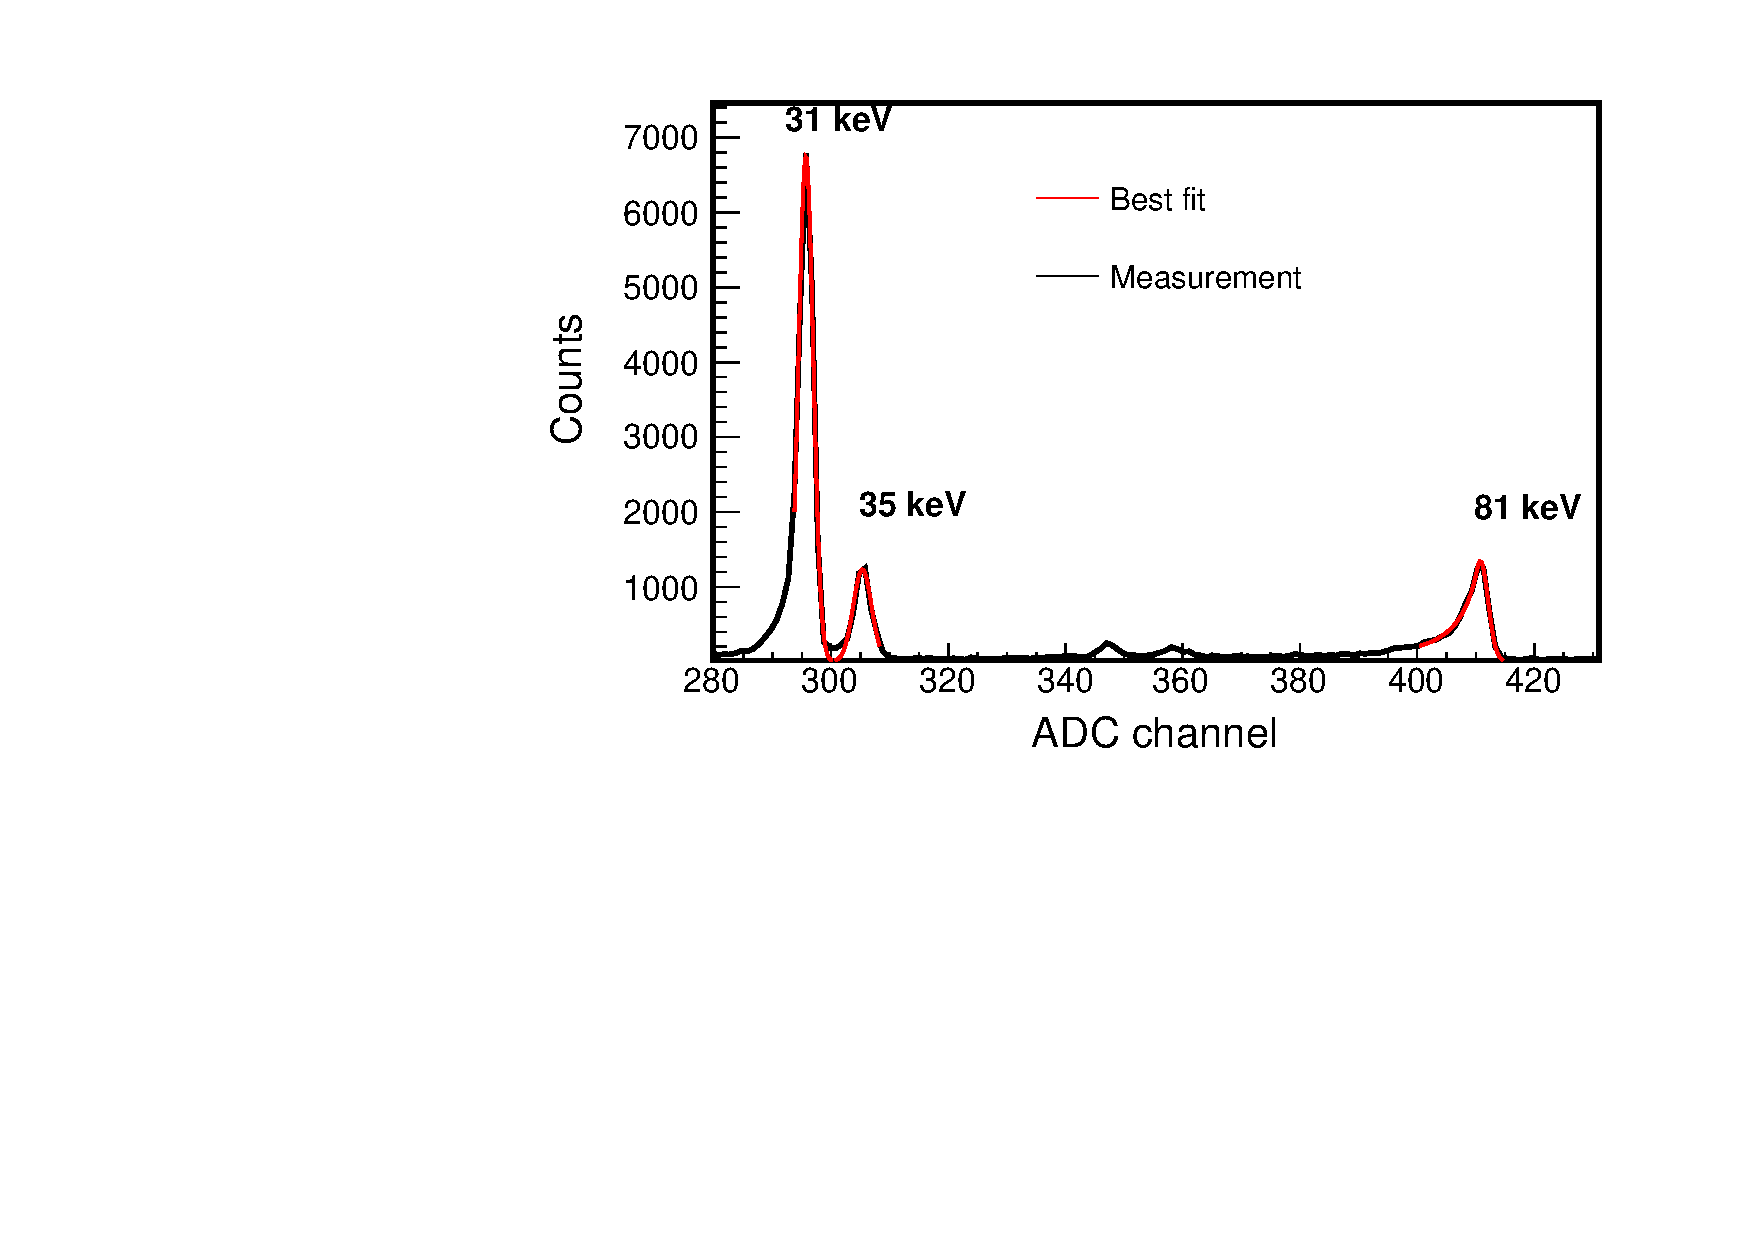
\includegraphics[width=0.8\linewidth]{figures/cal-fit.pdf}
  \caption{An example of STIX in-flight calibration spectrum.
  The most prominent peaks, from left to right, are photopeaks of 31 keV, 35 keV, and 81 keV
  photons. The first two peaks are fitted by the double-Gaussian function, and the high energy peak by  
  the crystal-ball function. }
    \label{fig:cal-fit}
\end{figure}
STIX converts ADC channels to "science energy channels" using an energy lookup table (ELUT) 
onboard by the FPGA, which defines the ADC channel edges  for each science channel for each pixel. 
A new ELUT is uploaded to STIX once a significant gain change is observed during the data analysis on the ground.  An EUT can be constructed using energy conversion factors determined from calibration runs. 
STIX continuously accumulates an  energy spectrum (in ADC units) for each pixel separately for events from the onboard Ba$^{133}$ sources and formats a  spectrum typically every 24 hours. 
The right panel of Fig.~\ref{fig:cal-fit} shows an example of the calibration spectrum with accumulation time of 24 hours.  The three most prominent peaks are produced by photons of 31 keV, 35 keV, and 81 keV photons from the calibration sources. To determine the positions of the photopeaks, the first two peaks are fitted with the double-Gaussian function, and the third peak with the crystal-ball function (\cite{crsystallball}),
which consists of a Gaussian core portion 
and a power-law low-end tail, below a certain threshold.
Then a linear line is fitted to the positions and the keV energies.  That gives the gain (i.e., the ADC to energy conversion factor) and baseline.
The ECC method (see \cite{ecc,ecc2})) is another method that the STIX team often uses to determine the calibration factors.  We found that the results of the two methods are consistent at 1$\sigma$.

The above steps are performed for each calibration spectrum once the data are available at the STIX data center. 
The calibration factors are written to a collection in the NoSQL database and used for further correction of energy bins in offline data analysis.   
Once significant changes in the calibration factors are observed, the STIX operations team creates a new ELUT and uploads it to STIX.

\subsection{Solar flare identification}
STIX identifies solar flares onboard on the basis of detector count rates, and the results are included in the QL data \cite{stix2020}.  However,  the data only provide limited information on flares due to the constraints of the telemetry budget and onboard computing resources.  Moreover, micro-flares are not reported due to the relatively high trigger threshold.
It is necessary to maintain a flare list on the ground for the needs of requesting science data and also for data users to find events of interest. 

\begin{figure}
  \centering
  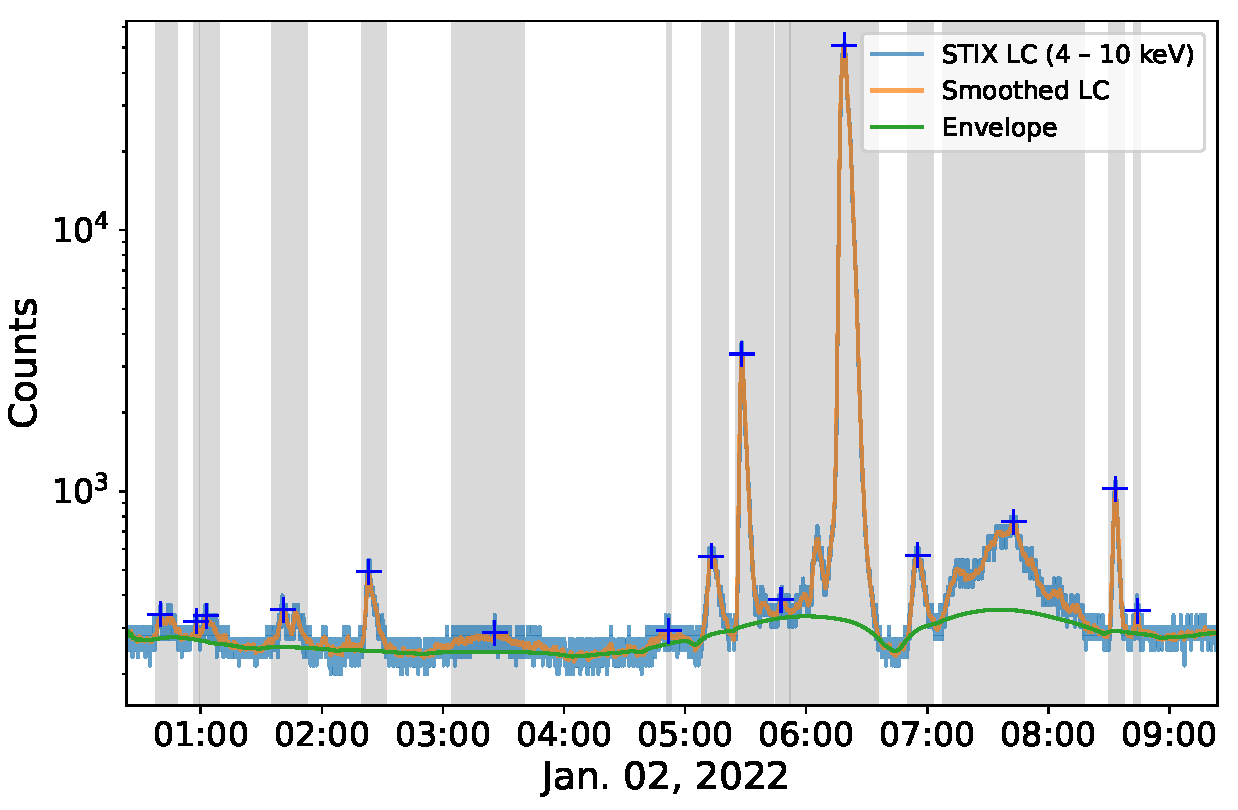
\includegraphics[width=0.8\linewidth]{figures/flaredet.pdf}
  \caption{STIX 4 -- 10 keV QL light curve recorded from 2022-08-10T21:00:00Z to 2022-08-10T18:00:00Z and  identified flares. The orange curve is the smoothed light curve using a moving average filter with a time window of 1 minute. 
  The identified peaks are marked with plus signs, and the colored ranges show their time ranges.
  }
  \label{fig:flare-det}
\end{figure}
Using QL light curves, solar flares can be identified in greater detail on the ground. 
The ground identification procedure includes the following steps:
\begin{itemize}
  \item Light curve smoothing: The selected light curve is filtered using an unweighted
  moving average filter with a time window of 1 min. This can smooth out statistical fluctuations and electric surge spikes;
  \item Envelope subtraction:  A flare may last hours, and there may be short-duration pulses lying on the envelope (the main pulse) in the light curve.  To facilitate the identification of those short-duration pulses, the envelope is subtracted from the smoothed light curve, which is estimated using the SNIP algorithm \cite{snip}. 
  \item Identification of flare peaks: We consider a flare is detected 
 if the peak count rate after envelope subtraction lies beyond two standard deviations 
 of the mean count rate during quiet Sun periods. 
  The flare start and stop times are given at the times crossing the threshold.  
  \item Merging of flare peaks: Two flares are considered as one single flare if their peak times differ by less than 5 minutes. This can reduce the number of flares reported and facilitate subsequent data analysis.  
\end{itemize}

As an example, Fig.~\ref{fig:flare-det} shows STIX QL light curve in the energy range 4 -- 10 keV, recorded from 2022-08-10T10:00:00Z to 2022-08-10T18:00:00Z.  The orange curve is the smoothed light curve.  The identified peaks are marked with the plus signs, and the colored ranges show the time ranges.

The above steps are repeated for QL light curves of the other four higher energies, which provide information on the upper limit of the X-ray energy of the flare.
The time ranges, peak count rate, and total counts as well as the corresponding ephemeris data of the identified flares are  stored in a collection called flare list in the NoSQL database.


\subsection{Solar flare standard analysis pipeline}
\subsubsection{Estimation of solar flare GOES class }
\begin{figure}
  \centering
  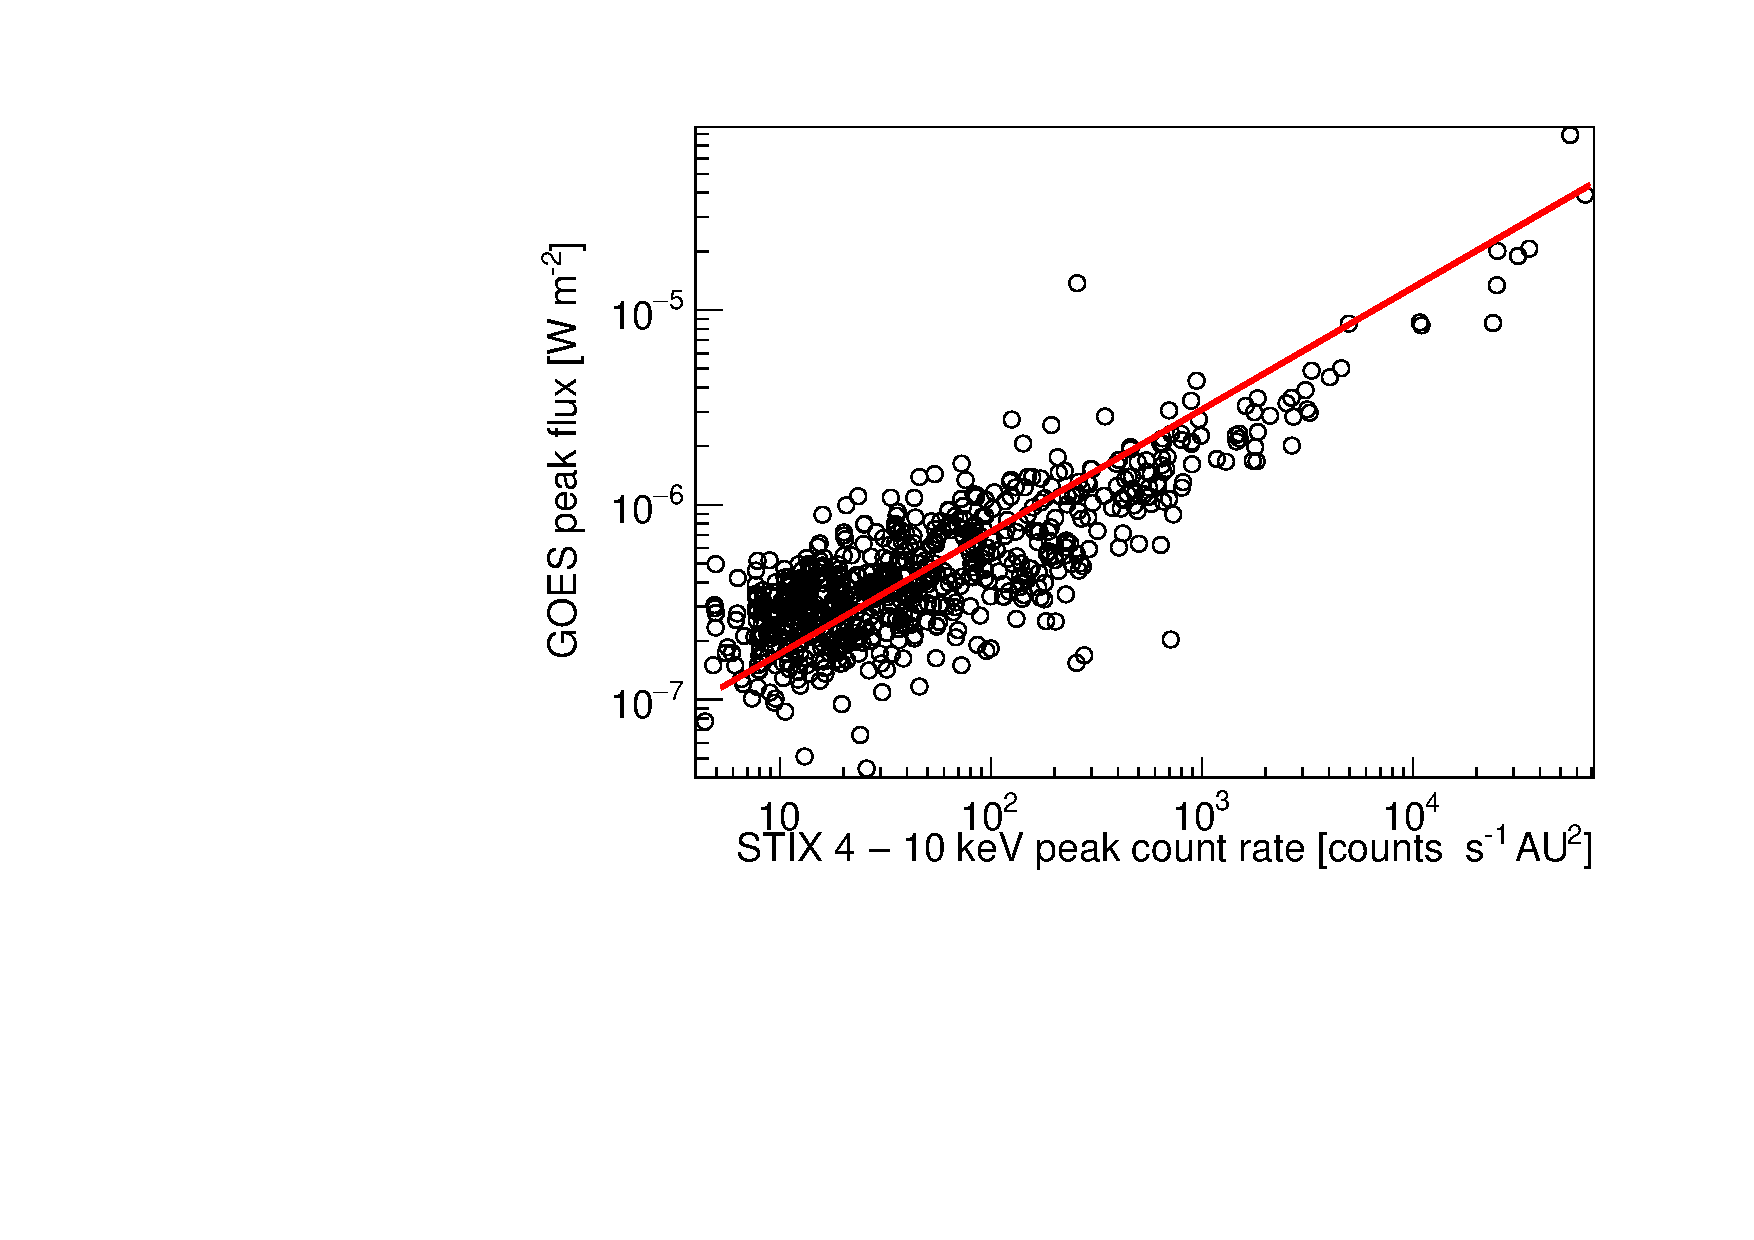
\includegraphics[width=0.8\linewidth]{figures/goes_stix_flux_paper.pdf}
  \caption{Scatter plot of GOES low channel peak flux with respect to the equivalent  peak count rate  at 1 AU  in the 4 -- 10 keV range for 717 solar flares observed by both GOES and STIX duration of the commissioning phase.   The solid line is a linear fit to the log-log graph. 
From the fit, we get the GOES flux estimation formula as follows:  $f = 10^{0.622 -7.376 \log_{10} (X^{'})}$ (in units of W/m$^2$),
where $X^{'}$ is the STIX peak count rate corrected for the distance variations between the Sun and Solar Orbiter. }
\label{fig:goes-stix}
\end{figure}
Solar Orbiter is far from Earth most of the time. 
Therefore, a considerable number of flares observed by STIX 
are not observed by GOES satellites (and vice versa). 
In order to estimate the GOES classes of such flares, 
we selected 717 solar flares observed by both GOES and STIX in 2021. 
Fig.~\ref{fig:goes-stix} shows the scatter plot of the peak fluxes
measured by GOES satellites with respect to the STIX background-subtracted count rates at the peaks, 
 in the energy range of 4 to 10 keV. 
STIX count rates have been corrected for 
the different distances between the Solar Orbiter and the Sun using $X^{'}=x r^2$,
where $X$ is the count rate after background subtraction
 and $r$ is the distance between the Sun and Solar Orbiter in units of AU.  There is a clear correlation between them, as can be seen in the figure.  The widespread at low fluxes can be explained by the difference in 
the energy response of the two instruments and the variation in flare temperatures. 
The correlation can be fitted with a linear fit in the log-log scale. 
From the fit, we get the GOES flux estimation formula as follows: 
$f = 10^{0.622 -7.376 \log_{10} (X^{'})}$ (in units of W/m$^2$), where $X^{'}$ is the STIX peak count rate corrected for the distance variations between the Sun and Solar Orbiter. It is currently used to estimate the GOES classes of flares that are not directly observed by GOES satellites.  The estimated GOES fluxes are stored in the flare list collection in the database. 

\subsubsection{Estimation of coarse flare locations using CFL data}
STIX estimates coarse flare locations onboard by 
maximizing the correlation between observed CFL pixel counts with expected counts using a lookup table \cite{stix2020}. 
With the requested science data, coarse flare locations can be reconstructed more accurately, as it allows for more sophisticated algorithms, greater flexibility in selecting time and energy range to be integrated, and more careful background subtraction.

When the pixel data of a flare is available at STIX center, its flare location is estimated. The steps are as below: 
1) Integrate counts around the peak for each CFL pixel. 
2) Subtract the background using a background file; and 3) estimate the illuminated area on each CFL pixel.  The estimation is based on two assumptions:  the illuminated area of a pixel is proportional to its relative count rate, and the total illuminated area of the imaging detectors is independent of the source location.
3) Estimated the flare location by minimizing the weighted sum of squared deviations (i.e., weighted chi-squares) between the calculated illuminated areas and expectations simulated for potential flare locations in a 400 $\times$ 400 grid.
\begin{figure*}
  \centering
  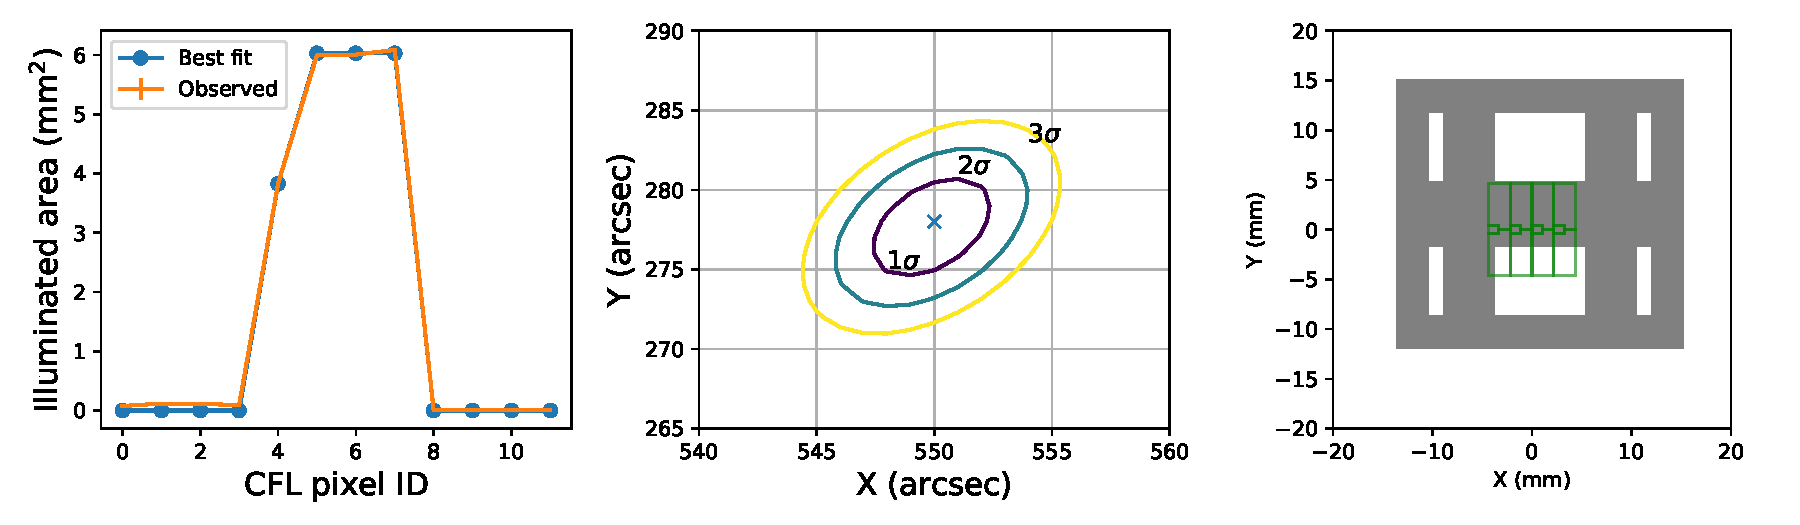
\includegraphics[width=0.95\linewidth]{figures/cflMay07.pdf}
  \caption{
   Left: Calculated areas of illuminated regions of 12 CFL pixels and the best fit simulated pattern for the flare location at (550, 278) arcsec. Pixels 0 to 3 are the top big pixels, Pixels 4 to 7 are the bottom pixels, and 8 to 11 are the small pixels as shown in the right panel.
   Middle: Best-fit flare centroid location (marked by x) and its 1$\sigma$, 2$\sigma$, and 3$\sigma$ confidence contours. Right: Projection of CFL sub-collimator (the gray shaded regions) on the detector simulated for the best-fit flare location. }
  \label{fig:cfl}
\end{figure*}
As an example, the left panel of Fig.~\ref{fig:cfl} shows the calculated and best-fit illuminated areas of the CFL pixels for the flare observed at 2021-05-07T19:00:00 (GOES class M3.9);  the middle panel shows the best-fit flare centroid location, as well as its $1\sigma$, $2\sigma$, and $3\sigma$ contours. 
The simulated CFL shadow pattern is shown in the right panel. 
Flare location sources are stored in the flare list in the database. 

\subsubsection{Imaging and spectroscopy pipeline}
\begin{figure*}
  \centering
  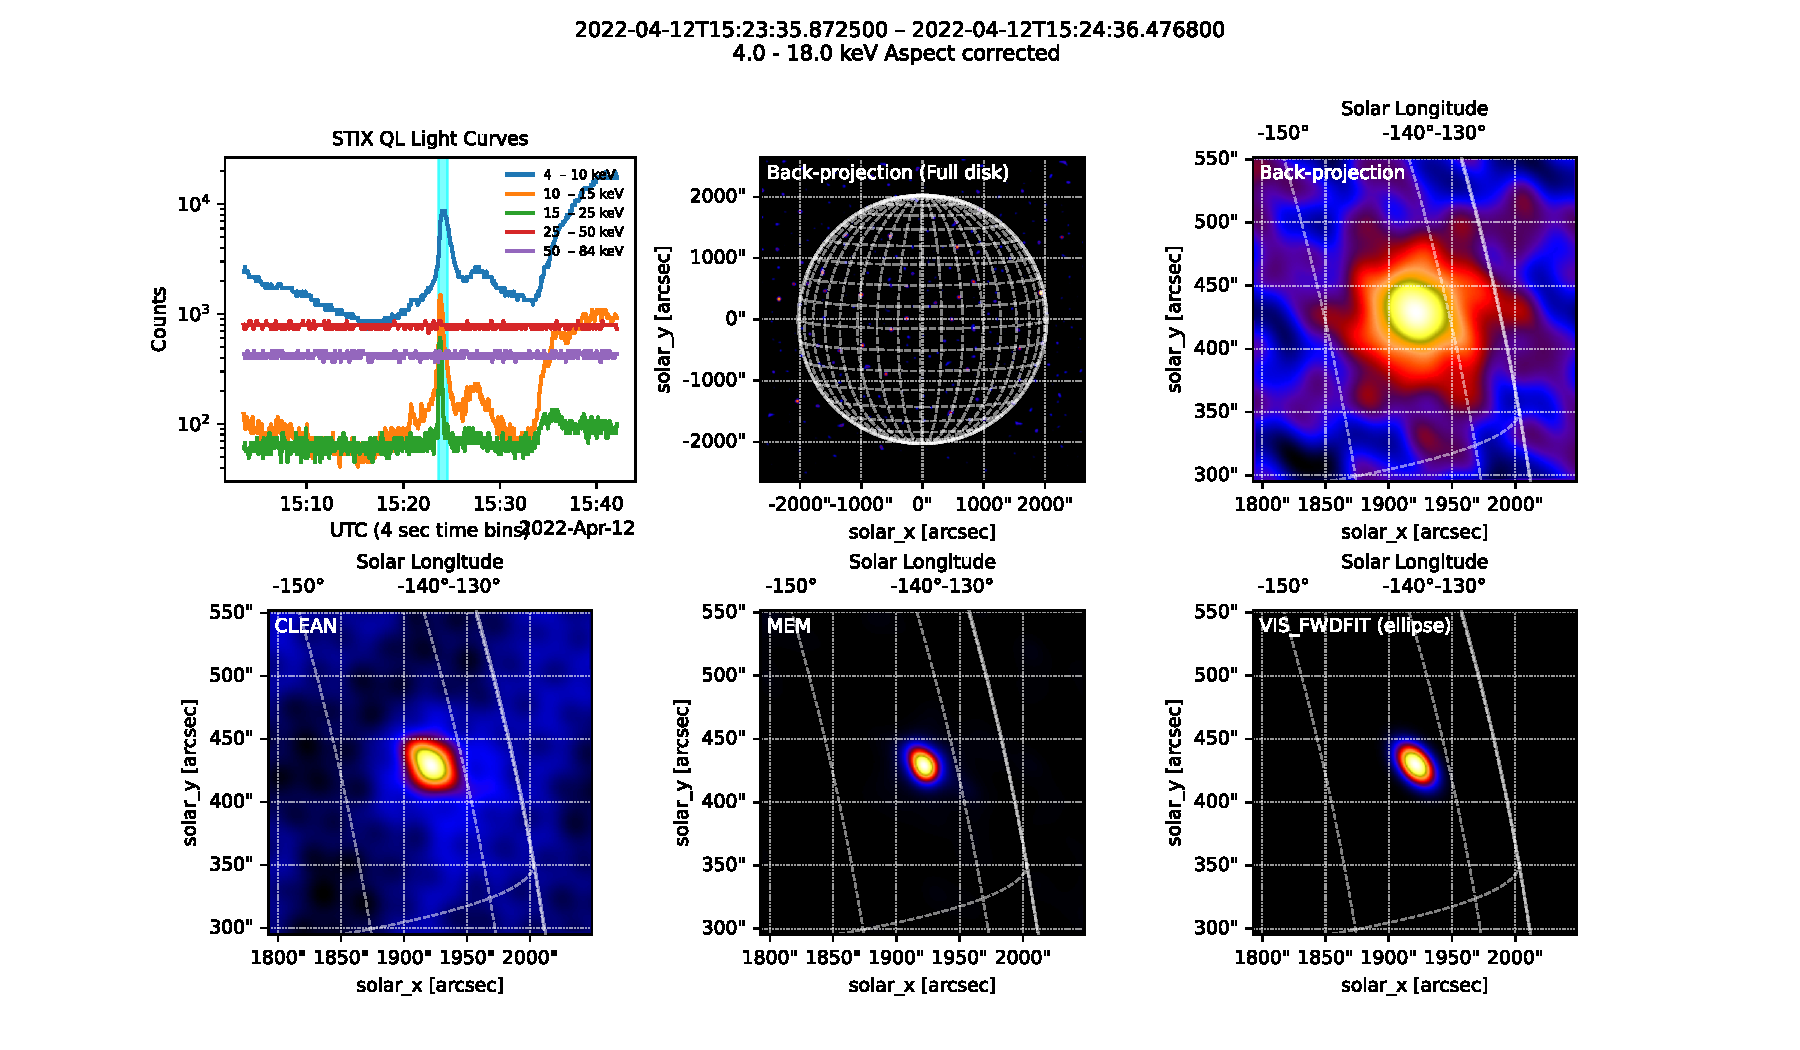
\includegraphics[width=0.95\linewidth]{figures/imaging_pipeline.pdf}
  \caption{ 
   STIX Quick-look light curves and reconstructed images of the solar flare observed at 2022-03-08T08:55:17Z, 
   created by the image reconstruction pipeline.  The period at the peak was selected and 
   Back-projection, CLEAN, EM, and VIS\_FWFIT
    algorithms were used for reconstructing images. }
  \label{fig:imaging}
\end{figure*}
STIX detects thousands of solar flares each year. However, only a small part of them is analyzed in detail by solar physicists. 
To help find flares of interest, we  developed an imaging and spectroscopy pipeline that automatically reconstructs images and perform spectral analysis for each ground identified flare after the reception of its pixel data. 

 For each flare, the pipeline first selects and integrates counts for 60 seconds around the peak of the flare for each pixel, then subtracts the background from the integrated counts using the pixel data acquired during a quiet solar period. 
 Subsequently, the transmission and dead time corrections are performed on the counts after background subtraction. The corrected counts are further converted into the visibilities of two energy bands of 4 - 10 keV (thermal energy) and 16 - 28 keV (non-thermal energy). 
Then the visibilities are used for image reconstruction using four different algorithms: back projection, CLEAN, MEM\textunderscore GE and VIS\textunderscore FWDFIT \cite{paolo2022,clean,mem}.
The reconstructed images are finally corrected  for STIX off-pointing and rotations. 
As an example,  the first panel of Fig. ~\ref{fig:imaging} shows the light curves and time range selected for a flare that occurred at 2022-03-08T08:55:17Z.
The rest of the panels show the images reconstructed with different algorithms. 
In addition to the image reconstruction, the counts after the transmission and dead time correction are used for spectral analysis.  Fig.~\ref{fig:ospex} shows an example of the spectral fitting results. The spectrum is fitted with a thermal component and non-thermal component ~\cite{andrea2021}. 

The results of the pipeline are saved to files in both FITS and PNG formats. At the same time, the file indexing information, parameter values from spectral analysis, and auxiliary data are written to a collection in the database. 


\begin{figure}[h]
  \centering
  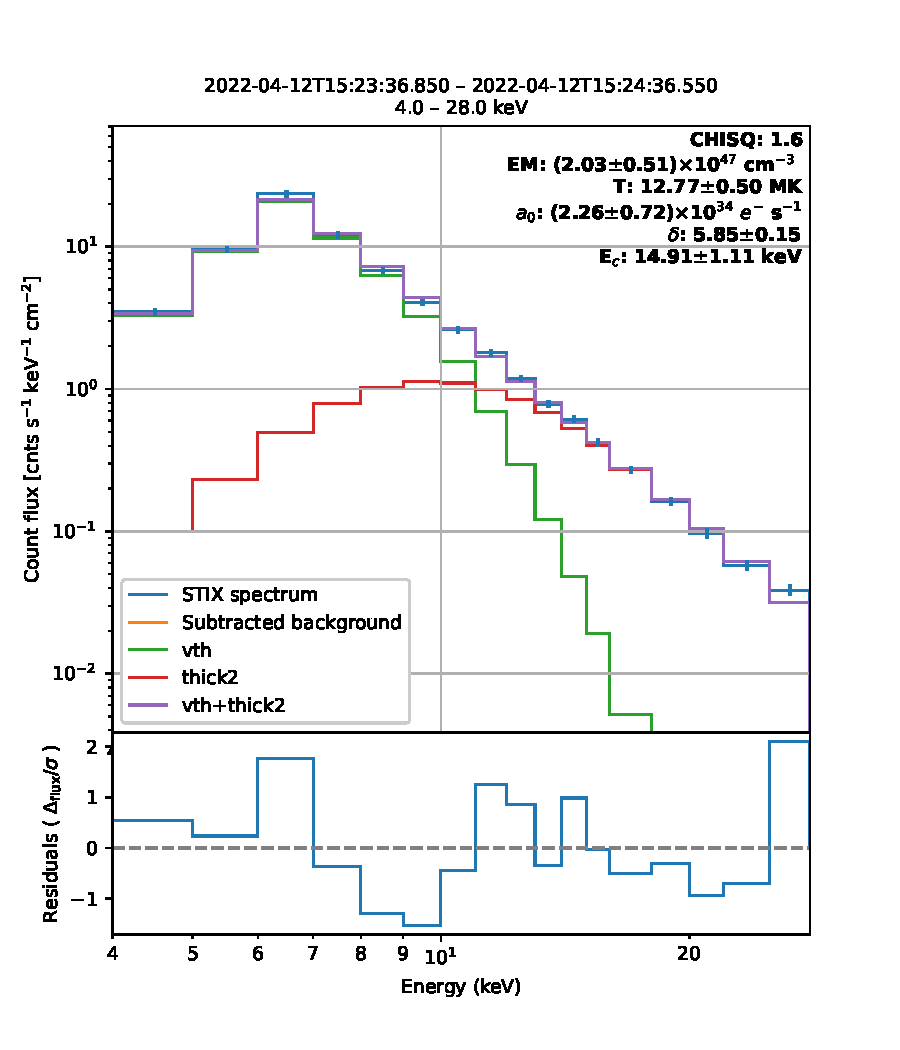
\includegraphics[width=0.9\linewidth]{figures/ospex.pdf}
  \caption{An example of spectral fitting results. 
    The imaging and spectroscopy pipeline performs
    spectral analysis for all flares in the flare list. }
  \label{fig:ospex}
\end{figure}
\section{Science data request strategy}
As mentioned earlier, the high-resolution pixel data are only downlinked in response to requests from the
ground. They are stored in the onboard archive memory for about four to six months 
before they are overwritten by new data. They are processed and downlinked 
after receiving data request telecommands from the ground. 
A data request telecommand contains information about the selected data and values of parameters  required to process the data onboard, including the data compression level, 
time range, minimal time bin, energy bin width, 
and  masks indicating detectors and pixels to be selected. 
STIX data detect thousands of flares per year; therefore, 
selecting data to be requested is a tedious task, as it must consider many factors
such as count rates, time binning of data, statistics of selected data, 
and also the telemetry budget when choosing values for the parameters. 
Over the past two years, the data selection strategy has been continuously optimized and the current strategy is: 
\begin{itemize}
  \item  
 Compression level-1 pixel data are requested for each of the ground-identified  flares with a total number of signal counts in the QL light curves greater than 10000, which is approximately the minimum counts to reconstruct an X-ray image. 
The requested energy range is chosen to be the range in which obvious signal counts are seen,  
whereas, the requested time resolution is adjusted based on the amount of data allocated. 
If the peak count rate is above 125 counts/sec (approximately 
equivalent to the count rate observed for a B3 flare at 1 au),  pixel counts with high time resolution are requested.  Otherwise, pixel counts are integrated over the whole flaring time 
to reduce the telemetry data volume. 
 \item  Spectrograms with the highest time and energy solution (compression level 4) are requested for all periods when STIX is in observation mode. 
 \item Time-integrated pixel data for background subtraction:
Time-integrated pixel data with durations of one or two detector temperature cycles (each cycle lasts about 40 minutes), which are acquired during quiet-Sun periods, are requested. 
The data are used for background subtraction when performing spectroscopy and imaging. 
\item High time-resolution aspect data are requested for periods when the aircraft's attitude changes drastically.
Such periods can be known from the SPICE kernels or the aspect system readouts in housekeeping data. 
\end{itemize}
Selecting the science data of the above types is done automatically using a program. The information of the selected data is written into a database collection.  Additionally, the STIX operations team also selects data for special 
needs.  After being checked and adjusted by the STIX operations team, groups of new data requests that meet the operations requirements are selected from the database and then compiled into instrument operation requests (IORs). 
IORs are used to create final telecommands at the mission operations center (MOC). An IOR is typically executed after two to three weeks of submission to ESA. 

\section{STIX data platform user interfaces}
\subsection{Interactive web pages}
\begin{figure}[h]
  \centering
  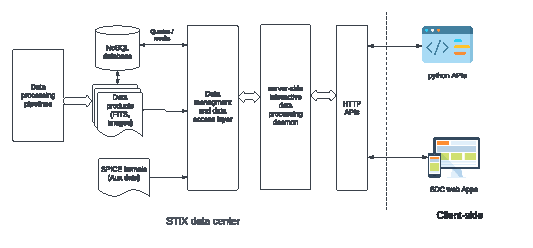
\includegraphics[width=0.9\linewidth]{figures/interfaces.pdf}
  \caption{ 
    Data flow at STIX data center.
  }
  \label{fig:interfaces}
\end{figure}

\begin{figure*}[h]
  \centering
  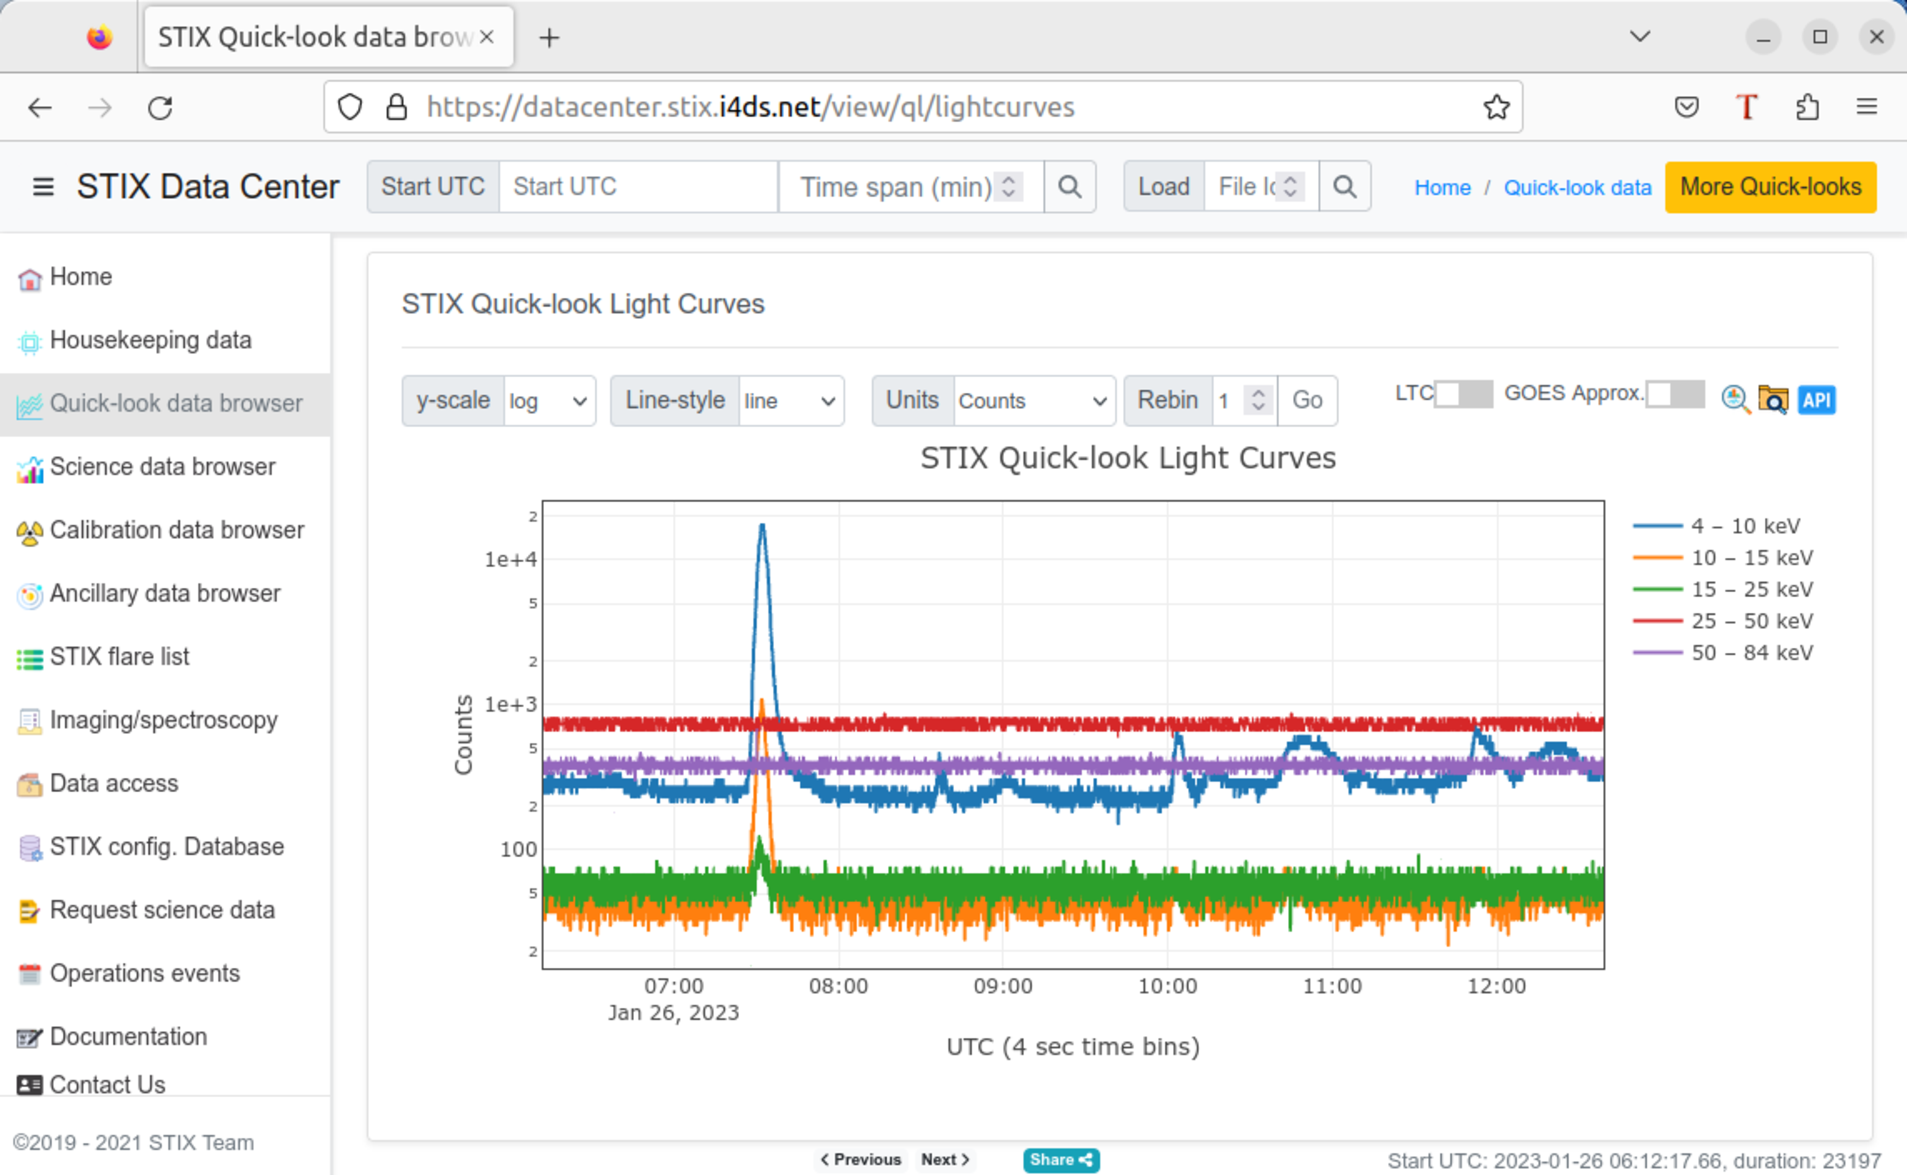
\includegraphics[width=0.7\linewidth]{figures/data-browser.pdf}
  \caption{ 
    Interactive web-based STIX Quick-look data browser. 
    In addition to STIX Quick-looks, it can also display quick-looks of simultaneous measurements 
    performed by other instruments, such as GOES X-ray fluxes, SDO/AIA images, and Solar Orbiter EUI. 
    The browser is available at the link \url{https://datacenter.stix.i4ds.net/view/ql/lightcurves}.}
  \label{fig:qlbrowser}
\end{figure*}
The data center provides various HTTP interfaces (APIs) that allow access to STIX data products
and the NoSQL database via HTTP requests. 
We have built dozens of web applications to manage and browser STIX data based on the APIs. 
Web techniques are chosen because they offer a number of advantages, such as clear cross-platform 
usability, broad access through browsers, rapid development, and easy maintenance.

As an example, Fig.~\ref{fig:qlbrowser} shows a screenshot of the STIX Quick-look data browsing 
tool. It allows users to browse available Quick-look data interactively. It 
interacts with the server through APIs. 
After receiving a request from the client side,
the server retrieves QL counts from the NoSQL database for the user-specified time range. 
After excluding duplicates and merging,  the server sends QL counts and metadata in JSON format back to the client. The data are then used to create interactive light curve plots using Javascript on the client side. 
The interactive plot uses state-of-the-art web technologies that enable users to perform a range of operations, such as rebinning the integration time, correcting the light travel time between the spacecraft and the Earth, and exporting data to a local file. In addition to STIX quick-looks, quick-looks from other solar-observing instruments can also be displayed on the same page after users' activation, 
making it easier to find events of interest for joint analysis.

Based on similar concepts, tens of web tools have been developed to browse other STIX data products.
The other four most commonly used tools are listed below: 
\begin{itemize}
  \item  Science data manager and browser.  It provides users with tools not only for visualizing science data, but also for searching, downloading, and analyzing science data. The interactive analysis tools allow users to interactively select data of interest for common analysis tasks such as background subtraction and energy rebinning,  without installing additional software. 
  The algorithms are implemented client-side using JavaScript. 
 Additionally, users can use the tools to submit imaging and spectroscopy tasks to the server and view the results on the same page. This reduces the barriers to exploring STIX data for new users and provides convenience for experienced users.

  \item  The preview images and spectroscopy product viewer is a web-based tool for managing and viewing the imaging and spectroscopy results. The viewer also provides also tools for, such as plotting the time evolution of emission measures and temperatures,  creating animations of x-ray images for the selected runs, and generating IDL or Python templates in order to reproduce the same results on  local machines.
  \item The auxiliary data viewer is a tool that allows the user to view auxiliary data, such as the locations of the spacecraft, its velocity, and its attitude. The viewer uses data derived from the SPICE kernel or from aspect system readouts stored on the server side.  The viewer also provides tools to calculate the looking angle of flares and the coordinates of solar limbs in STIX FOVs.
  \item  With the housekeeping browser, users can view time-series plots of all STIX housekeeping parameters, including the temperature, voltage, operation mode, memory status, etc. It provides great convenience for the instrument operations team to monitor the instrument status. 
\item 
The STIX data access page offers users a variety of tools to search and download STIX FITS products. 
It also provides links to tools for previewing the products. As soon as they are generated at the STIX data center, STIX data products are immediately available for access on the page.
\end{itemize}




\subsection{STIX data center interface:  stixdcpy}
{\it stixdcpy} is a python package that facilitates accessing and analyzing stix data. 
With {\it stixdcpy}, users can easily query and download the data products available at the STIX data center.
Similarly to the web tools, stixdcpy also provides tools to perform some common analysis of STIX data, such as dead time correction, transmission correction, data clipping, and merging. 
{\it stixdcpy} is still under active development. 
As a result, its features and 
capabilities may change over time.  The source code of {\it stixdcpy} is hosted on the GitHub repo at \url{https://github.com/i4Ds/stixdcpy}.
\section{Summary}
\label{sec:summary}
STIX is one of ten instruments onboard the Solar Orbiter, 
which was launched into space on February 10, 2020.
 STIX measures the spectrum and takes X-ray images of solar 
 flares in the energy range of 4 -- 150 keV.  
 During nominal operations, STIX continuously generates telemetry data. 
 To process and archive the data as well as to support the operation of 
 instruments and scientific activities using STIX data, 
 dedicated data processing pipelines and a data platform have been 
 developed for STIX.
 The pipelines generate telemetry at different levels and perform common scientific analyses. 
 The platform provides 
 all STIX data products of different levels and also provides users 
 with various web-based tools for searching and browsing STIX data products. 
 It also provides web-based tools to perform common analysis tasks with STIX data. 
  The data center is designed to work in a 
 fully automatic mode with minimal human intervention. The concept has proven successful 
 and has been running continuously for more than two years.
The platform not only facilitates the operations of the instrument but also provides great support to STIX data users.



\bibliographystyle{aa}
\bibliography{citations}

\end{document}
%data records, documentsMongoDB is a type of NoSQL database that uses a document-oriented data model. 
%This means that data is stored in the form of documents, which are similar to JSON objects. These documents are organized into collections, %which are similar to tables in a relational database. A MongoDB database can contain one or more collections, and each collection can contain %any number of documents.